\documentclass[letterpaper,12pt]{article}
\usepackage{lineno}
\usepackage{times}
%% Indent length
\usepackage{indentfirst}
\usepackage{graphicx}
\usepackage[margin=1in]{geometry}
\usepackage[singlespacing]{setspace}
\usepackage{hyperref}
\usepackage{wrapfig}
\usepackage{pgfgantt}
\usepackage{enumitem}
\usepackage{caption}
%BiB
\usepackage[sort&compress,square,comma,authoryear]{natbib}

\usepackage{titling}
\newcommand{\advisor}[1]{%
  \postauthor{%
    \end{tabular}\par\end{center}
    \begin{center}\large Advisor: #1\end{center}
  }
}

%The proposal should include:
%a statement of the problem to be investigated, its background and significance approach(es) to be followed for its resolution, preliminary results, anticipated timetable for completion, pertinent bibliography. 

%The proposal should specifically document the anticipated contribution that this work will have to the body of knowledge. 

%A separate page listing the proposed title, author’s name, Research Advisor’s name and an abstract of no more than 350 words must also be submitted. 
%The preferred format is similar to that of proposals submitted to a Federal Agency. There is a 15 pages (single space, 12 point, Arial) limit on the scientific portion of the proposal. This includes tables and figures but does not include the bibliography. Please refer to the template. Students must distribute their prospectus to their committee members a minimum of three weeks ahead of the anticipated oral prospectus presentation date.

% The title page should contain the proposed title, author’s name, the research advisor’s name and an abstract  of  no  more  than 350 words

\title{Remote sensing of small-scale ionospheric turbulence: GNSS phase scintillation imaging}
\author{Sebastijan Mrak}
\advisor{Prof. Joshua Semeter}

\linenumbers*[1]

\begin{document}
\maketitle
\thispagestyle{empty}
\begin{abstract}

Earth's upper atmosphere is a tightly coupled and dynamic electric circuit, whose most prominent manifestation is the aurora. During space weather events, the Earth's atmosphere is bombarded by an enhanced flux of energetic charged particles from the magnetosphere. This ionizing flux creates steep gradients and turbulence in the ionospheric plasma, which alters the state of the system. The modified electrodynamics can drive the ionospheric plasma unstable, causing small-scale transient structures, which alter the circuit current closure and trans-atmospheric radio signals.

The resulting plasma irregularities have small spatial and short time scales, making them challenging to observe. In fact, there is no established remote sensing technique that is able to fully resolve them. Hence, their spatiotemporal extent and their physical origin remain open scientific questions. At the same time, the  plasma turbulence severely alters global navigation satellite system (GNSS) signals; distorting their positioning and timing solutions. We propose to utilize these fluctuations in the GNSS signals, measured by dense networks of ground-based receivers, to reconstruct the plasma dynamics, thus leveraging GNSS infrastructure as a massive opportunistic space weather observatory. 

Preliminary results using a regional receiver network have revealed new constraints on the spatiotemporal occurrence of signal fluctuations, and new insight into observability of this physics for a given sensor topology. We propose to build upon these results to create a continental-scale imaging tool for studies of ionospheric turbulence.  The multi-scale measurements enabled by the envisioned system will lead to new insight into the formation and consequences of small-scale  turbulence.  The proposed GNSS phase scintillation imaging tool presents a framework for new understandings in resolving magnetosphere-ionosphere interactions,   associated ionospheric electrodynamics, and effects on GNSS positioning capabilities. 

\end{abstract}
\clearpage
\setcounter{page}{1}
% ---------------------------------------------- INTRO ----------------------------------------------- %
\section{Introduction}

The Earth's ionosphere is a natural plasma laboratory that acts as the Earth's system sensor to extraterrestrial and terrestrial forces. Continuous solar irradiance modulates the ionospheric plasma by means of plasma production on a daily basis. Conversely, intermittent solar events, such as solar flares and coronal mass ejections, stir the ionospheric plasma in unpredictable ways. Unlike the periodic behavior, the latter transient modifications affect human society by means of inducting lithospheric currents, geoelectric fields, altering trans-atmospheric radio-wave communications. The global navigation systems became an invaluable asset the human society relies on, engineered to enable precise positioning and time reference. However, the transient ionospheric irregularities, peculiar to high latitude ionosphere, distort the integrity of GNSS service. Normally, we endeavor to mitigate such predicaments by means of engineering mitigation techniques, however, one can utilize the altered radio waves as a diagnostic of the transient plasma irregularities. In this prospectus, we introduce a novel GNSS-aided engineering asset for advancing fundamental knowledge of the magnetosphere-ionosphere (MI) coupling physics.

It has been found that ionospheric irregularities play an important role in closing the geospace electric circuit. The ionosphere can be thought as a spatiotemporally variable impedance load to a geospace circuit, and an irregular medium for traversing radio waves. The ionosphere closes magnetospheric current system in a collisional domain (D/E region ionosphere), where electrodynamic processes can drive the plasma unstable and consequently alter the ionospheric current system. The resulting non-linear effects heats up the plasma \citep{Dimant2003} and impose a non-linear current \citep{Dimant2011a, Dimant2011b}, which alters the ionospheric conductivity, and hence the energy dissipation. \citet{Wiltberger2017} implemented the latter suggestions into a global MI model, and found a huge improvement in a modeled substorm polar cap potential, geomagnetic indexes and the total energy budget. On the other hand, the plasma instabilities constitute regions or highly dynamic and transient electron density irregularities, causing radio waves to refract and diffract. At high latitudes, the refraction is predominant~\citep{Spogli2009, Jiao2013}, hence the fluctuations cause navigation positioning distortion~\citep{Jacobsen2016}, and loss of the signal~\citep{Semeter2017}, despite the signal strength remains unaffected.

Inherent multi-frequency GNSS operation enable estimation of the Total Electron Content (TEC) along the signal's path, by virtue of utilizing a dispersive nature of the plasmas. The absolute value of TEC can be estimated \citep[e.g.][]{Rideout2006}, and such maps led to a handful of important scientific discoveries \citep[e.g.][]{Foster2002, Foster2005}. However, the TEC maps of absolute TEC are an inadequate tool for identification and diagnostic of small-scale and transient plasma features. \textbf{The high latitude ionospheric irregularities have short time and small spatial scales, making them extremely challenging to observe. In fact, no classical remote sensing technique is able to fully resolve them.} Actually, there is no quantitative assessment of the small-scale forcing contribution to a global energy budget. GNSS signals are corrupted by transient, small-scale plasma irregularities, which suggest the GNSS as a possible opportunistic remote sensing diagnostic for the plasma turbulence. \textbf{Therefore, we propose to construct a novel GNSS imaging tool, utilizing the scintillating phase as a diagnostic of small-scale ionospheric disturbance.}

Electrodynamics, density gradients, flow shears, peculiar to high latitude ionosphere produce irregularities that predominantly refract the GNSS signals. While recent observations led to new understandings in scintillation climatology~\citep{Spogli2009, Prikryl2011, Jiao2013}, \textbf{the physical mechanisms, spatiotemporal evolution and their direct relation to the MI coupling remains unresolved}. This proposal is motivated by recent results~\citep{Semeter2017, Mrak2018mahali} enabled by a dedicated $\sim$15~km baseline GNSS receiver array deployed to central Alaska~\citep{Viktor2014}. The findings are summarized as: \textbf{(i) phase scintillation regions are adjacent to auroral arcs; (ii) plasma instabilities most reside in the ionospheric E- region; (iii) electrodynamics and density gradients are most likely drivers for causative instabilities.} In addition, the latter campaign revealed important remote sensing observational constraints: \textbf{(I) Geometric constraints in a 2D projection plane; (II) Aspect angle dependence of the phase scintillation; (III) Transient and small-scale nature of the irregularities.} 

GNSS receivers are sensitive to tiny fluctuation in the signal's phase, caused by the ionospheric plasma, which is a definition of an opportunistic space weather remote sensing observatory. In this proposal, we emphasize the outstanding scientific questions we aim to address, provide a synoptic description of the methodology, and work in progress. \textbf{The anticipated contributions of the proposed work are: (a) Continental-scale phase scintillation maps: a proxy indicator of small-scale plasma turbulence occurrence; (b) a multi-sensor data fusion: resolving small-scale features in a context of meso-scale optical aurora; (c) development of optimal strategies for extracting physical parameters form GNSS signals.} In a broader context, the proposed research will foster a nowcating maps of GNSS positioning distortion, a service provided by the Space Weather Prediction Center (SWPC).

% --------------------------------------- Objectives ----------------------------------------- %
\section{Research Objectives}

As outlined above, high latitude ionosphere is extremely dynamic and peculiar plasma environment, controlled by the MI interaction. Small-scale transient phenomena alters the geospace current system in unpredictable ways, and no established remote sensing tool is capable to fully resolve them. We emphasize three outstanding scientific questions we aim to address:
\vspace{-0.5em}
\begin{enumerate}
\item \textbf{How do the MI-coupling geometry constraint observability of the system, as seen from ground-based remote sensing point-of-view, and how do we mitigate it in order to fully exploit the sensor's field-of-view?}
\vspace{-0.5em}
\item \textbf{What is the spatiotemporal distribution of the plasma turbulence with respect to the optical aurora? How does the distribution affect the total energy budget of the MI-system?}
\vspace{-0.5em}
\item \textbf{Which physical processes are responsible for the causative plasma irregularities, and what is their dependence on the geophysical drivers?}
\end{enumerate}
% ----------------------------------- Methodology ----------------------------------------- %
\vspace{-1.5em}\section{Methodology}

The raise of the global navigation systems began in early 1990s with the Global Positioning System (GPS) and Russian GLONASS. The navigation satellites are deployed in the middle Earth orbit ($\sim$20,000~km) with an orbital period of $\sim$12~hours. All navigation systems inherently operate at at least two frequencies (L1$\sim$1.6~GHz and L2$\sim$1.25~GHz)) to mitigate ionospheric delay. Most of the currently operating GNSS receivers only supports the GPS constellation, nevertheless, even at high latitudes  each receiver sees at 5-7 satellites at all times. The number of the GNSS receiver is ever increasing, primarily for the purposes of geodesy, transportation and robotic farming. The GPS has several practical advantages over the GLONASS for the geophysical purposes, therefore most of applications were build solely with the GPS signals. Recently, European GALILEO and Chinese BEIDOU became operational, and are being integrated in the geoscience. Altogether, the GNSS has now more than 80 operational satellites. Therefore, a systematic use of the available resources with a state-of-the-art data processing strategies, enabled by a capability of tracing many satellites by each receiver simultaneously, define an invaluable remote sensing asset for geophysical purposes. 

\begin{wrapfigure}[15]{l}{0.65\textwidth}
\centering
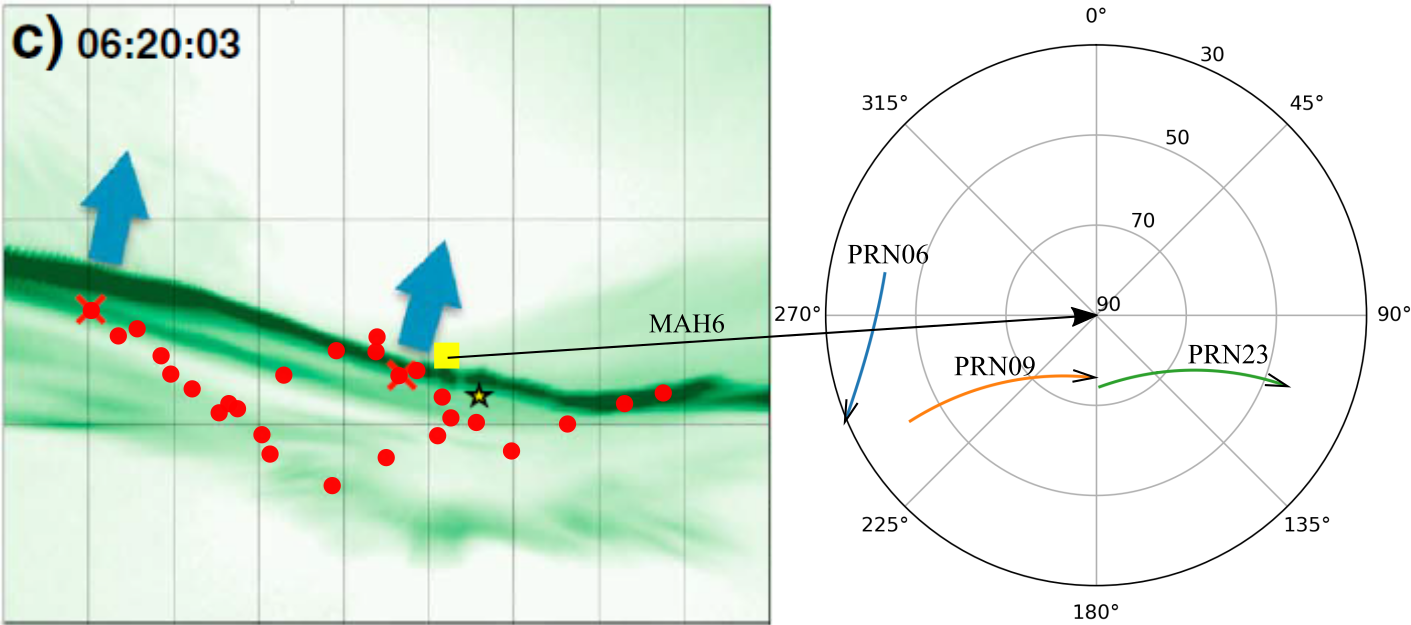
\includegraphics[width=.6\textwidth]{fig/mahali-map-orbits.png}
\caption{An example of traversing discrete aurora over a GPS receiver array field of view. Red circles denote piercing points closest to the optical structure, utilizing three GPS satellite-receiver lines of sight.}
\label{fig:mahli-aurora}
\end{wrapfigure}

For practical reasons, we focus our discussion of technology demonstration only for the GPS case. An example map of GPS observations, probing discrete aurora is depicted in Figure~\ref{fig:mahli-aurora}. We utilized a small baseline array of GPS receivers, and only three of the available lines-of-sight. The illustration shows a particular advantage of GNSS remote sensing: a great spatial coverage, enabling to sample the aurora with unprecedented space--time resolution.

% -------------------------------------------- GPS -------------------------------------------------- %

\vspace{-1em}\subsection{Technical background}
A GNSS receiver continuously measure received power $S$ and phase $\Phi$, where the phase can be the one of the pseudo-random code (normally in units of length) $P$, or a phase of the corresponding wave carrier $L$. Pseudo-range is the fundamental measure of satellite navigation system, used to estimate the distance between a satellite and the receiver, and hence to compute a navigation solution. However, variance of the measurement depends on the wavelength. For the Global Positioning System (GPS), the L1 (1575.42~MHz) civil code length is 1023~bit, transmitted at 1.023~Mbit/s, namely the length of a single bit in a vacuum is $\sim$293~m. On the other hand, the wavelength of the L1 carrier is $\sim$0.19~m, hence the carrier phase information provides more accurate measurements~\citep{Coster1992, Coster2012}.

Radio-wave propagation in a presence of a dielectric medium is retarded proportionally to its refractive index. The permittivity of plasmas is a function of the probing frequency (dispersive medium), moreover the ionospheric plasma is only partially ionized. Its refractive index is fully described by the Appleton-Hartree equation \citep{Appleton1932}. However, due to the fact the plasma frequency $\omega_p$ is much bigger than plasma gyrofrequency $\Omega$ and collision frequencies $\nu$, one can neglect contributions of the latter ones~\citep[cf.][]{Kashcheyev2012}. The ionosphere is a highly dynamic plasma ecosystem, hence its index of refraction $n(\textbf{r},f,t)$ is a function of the position $\textbf{r}$, time $t$, in addition to the probing frequency. The simplified expression for refractive index of the plasmas $n$ is:
\begin{equation}
n(\textbf{r},t) \approx 1 - \frac{n_e(\textbf{r},t) e^2}{2 \epsilon_0 m_e (2\pi)^2 f^2} \approx 1- \frac{40.3}{f^2} n_e(\textbf{r},t)
\end{equation}
where $n_e(\textbf{r},t)$ is a plasma electron density at a position \textbf{r} and time $t$, $e$ is the charge of an electron, $\epsilon_0$ permittivity of the free space, and $m_e$ mass of an electron. Total phase $\Phi$ of the traversing electromagnetic wave of a given frequency $f$ between a satellite and a receiver is:
\begin{equation}
\Phi = \int_0^L n(\textbf{r},t) dl = \int_0^L \left(1 - \frac{40.3}{f^2} n_e(\textbf{r},t)\right) dl = \Phi_0 - \Phi_i ~ [m]
\label{eq:phase}
\end{equation}
where the integral $\int_0^L n_e(\textbf{r},t)~dl$ represents an integrated plasma density along the receiver-satellite line-of-sight $l$, or the total electron content (TEC) in units of $el^-/m^2$. $\Phi_0$ is the receiver-satellite geometric distance (in units of meters), and $\Phi_i$ is the ionospheric correction due to altered speed of propagation. Further, the refractive index $n$ of plasmas is less than 1, the phase velocity is intrinsically larger than the speed of light, and hence the plasma inducts a phase advance to the carrier phase. Conversely, group velocity in plasmas is smaller than the speed of light. For certain applications, we only care about relative fluctuations in the signal's phase, therefore we can rewrite the equation~(\ref{eq:phase}) to:
\begin{equation}
\Phi = \Phi_{DC} + \Delta\Phi
\end{equation}
where $\Phi_{DC}$ denotes a baseline receiver phase that encompasses the actual range with additive slow variations, whereas $\Delta\Phi$ are variations around the baseline. Therefore, we assume it is possible to extract only spatiotemporal fluctuations $\Delta\Phi$ inducted by the ionosphere, if we are able to deconvolve them from the background $\Phi_{DC}$. Further consideration of the ionospheric modulation $\Delta\Phi$ can be written as:
\begin{equation}
\Delta\Phi =- \frac{2 \pi 40.3}{c_0 f} \Delta TEC ~[rad].
\end{equation}
$\Delta\Phi$ therefore depends solely on the changes in integrated electron density $\Delta TEC$, hence we postulate it is possible to utilize the GNSS measurements of the received phase to identify plasma irregularities (i.e. changes in TEC). However, one has to bear in mind that a single frequency measurements are ambiguous by the fact one is unable to isolate the system contributions of the measured phase, and to identify the baseline TEC value. Hence, dual frequency approach for an absolute measurement is necessary to unambiguously resolve them~\citep[cf.][]{Coster1992, Rideout2006}. 

\vspace{-1em}\subsection{GNSS data processing}

\begin{figure}[h]
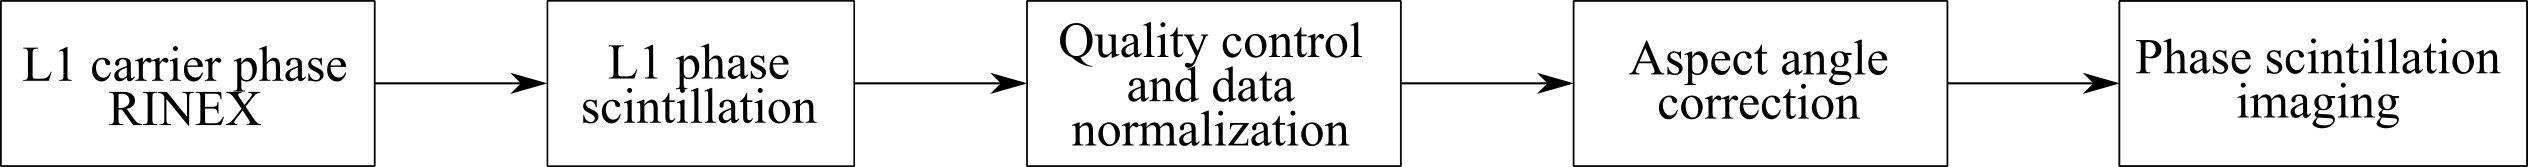
\includegraphics[width=\textwidth]{fig/work-flow}
\caption{Proposed work flow diagram for end-to-end signal processing.}
\label{fig:work-flow}
\end{figure}

The proposed signal processing flow diagram is depicted in Figure~\ref{fig:work-flow}. Observations from available repositories come in compressed ASCII Receiver Independent Exchange Format (RINEX) or manufacturer-specific binary files. The data will be first converted into a standardized RINEX format, and then converted\footnote{https://github.com/aldebaran1/georinex} in a database-like multidimensional array, prepared for the further processing. 

\begin{wrapfigure}[26]{r}{0.5\textwidth} %First optional argument = number of lines
\vspace{-1em}
\centering
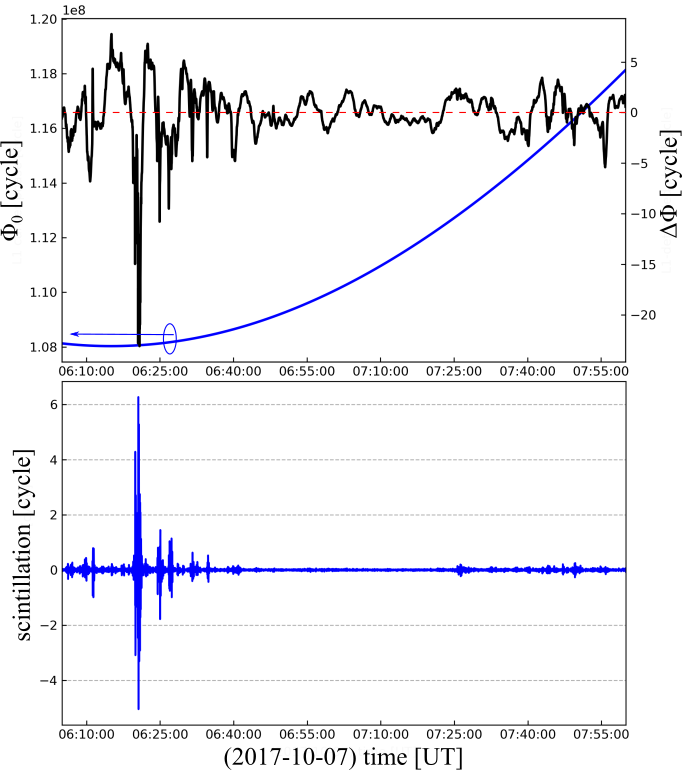
\includegraphics[width=.48\columnwidth]{fig/range-phase-scint}
\caption{An example of GPS observations during a substorm expansion event. (top panel - blue) Carrier phase (L1) measurements of satellite PRN23 in units of cycles; a proxy measure of the receiver-satellite distance $\Phi_0$. (top panel - black) Detrended carrier phase measurements, showing variations of the received phase $\Delta\Phi$. (bottom panel) Phase scintillation: high-pass filtered $\Delta\Phi$.}
\label{fig:phase-scint}
\end{wrapfigure}
The data processing is segmented into four basic operations. First, line-of-sight phase scintillation time-series is computed, then the data validation and classification is taking place. The line-of-sight observables will converted to a "vertical" (normalized) phase scintillation, according to the geomagnetic aspect angle correction (mapping function). Finally, data from multiple receivers and all available lines-of-sight will be combined into 2D maps of plasma turbulence. Each step in the diagram is discussed in greater detail.

\vspace{-1em}\subsection{Phase scintillation}

Figure~\ref{fig:phase-scint} depicts an example measurement of the received L1 carrier phase (top panel - blue line). The observable is a proxy receiver-satellite range measurement, hence the parabolic shape. The apex represents a position in space and time, where the satellite was at the closest approach to the receiver. Therefore, this measurement can be also thought as the zeroth order approximation of the $\Phi_{DC}$. The units of phase are measured in cycles, however the absolute value (geometric range) is ambiguous, due an arbitrary phase at the very beginning. 

We adopt a standardized routine to extract high frequency fluctuations, that is phase scintillation, ~\citep{Mitchell2005, vanderMeeren2015, Mrak2018mahali}, utilizing polynomial detrending, followed by a sixth-order Butterworth high-pass filter. In the Figure~\ref{fig:phase-scint}, we illustrate this process by showing phase variations around a baseline, as previously defined $\Delta\Phi$, depicted with the black curve (top panel). The variations around the zero crossing can be explained as follows: negative perturbations represent electron density enhancements, which increase propagation velocity. Conversely, positive variations resemble regions of plasma depletion. High-pass filtering is then applied to the $\Delta\Phi$ signal and the resulting high frequency fluctuations (i.e., phase scintillation) are depicted in the bottom panel. The outlined processing has already been developed and is under continuous integration\footnote{https://github.com/aldebaran1/pyGnss}.

\vspace{-1em}\subsection{Data validation}

We propose to exploit the GNSS carrier phase measurements into scintillation maps, which implies simultaneous use of all available observations. This requires a rigorous data validation, in order to avoid nonphysical interpretation of possible systematic or processing artifacts. Figure~\ref{fig:phase-signature} depicts a phase scintillation event caused by multiple auroral electrojet intensifications. Figure shows detrended L1 carrier phase measurement (blue) and the corresponding phase scintillation component (black line). The figure illustrates three important questions we need to embed in the data validation routine:
\begin{enumerate}[leftmargin=*]
\vspace{-0.5em}
\item How to validate the origin of the scintillation events. Is the origin ionospheric or is it caused by a systematic error?
\vspace{-0.5em}
\item How to interpret phase scintillation signatures (validated) in terms of the physical origin.
\vspace{-0.5em}
\item How to extract and optimally represent physically meaningful information in a 2D maps; measurements with an arbitrary phase, aspect angle, and measured by different receiver hardware?
\end{enumerate}

\vspace{-0.5em}
\begin{wrapfigure}[17]{r}{0.5\textwidth}
\vspace{-1em}
\centering
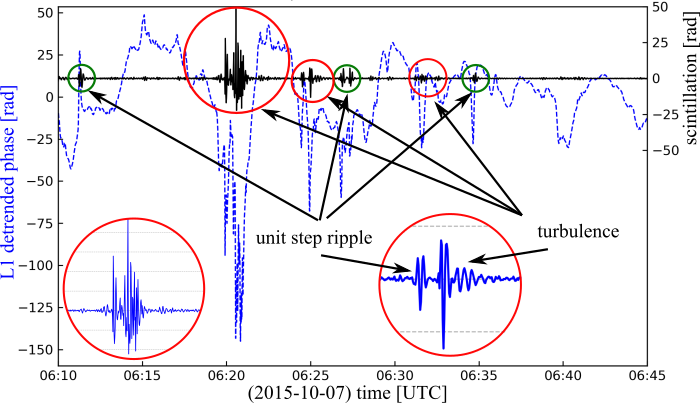
\includegraphics[width=.48\textwidth]{fig/L1-turbulence}
\caption{L1 phase measurements and interpretation. Detrended L1 carrier phase (blue line) and high pass filtered (scintillation) in black line. Two types of scintillation signature are marked in red and green, representing turbulence and unit response (respectively).}    
\label{fig:phase-signature}
\end{wrapfigure}
Formulae of the resulting phase variations $\Delta\Phi$ (Eq.~\ref{eq:phase}) is straightforward, however, it is deceiving by the fact the total measured phase is a convolution of systematic (hardware), and atmospheric contributions. Moreover, the detrending process uses an arbitrary baseline polynomial: therefore one cannot equate the changes in L1 direct to the change in the plasma electron density. %A more general interpretation of phase signature (Figure~\ref{fig:phase-signature} - blue line) is however valid: negative perturbations resemble a shorter receiver-satellite distance owing to increased phase velocity, hence the plasma density enhancement. Likewise, the positive deviations resemble plasma density depletions.

A more unambiguous, but limited interpretation can be told through the phase scintillation point-of-view. Figure~\ref{fig:phase-signature} (black line) shows characteristic signatures at high latitudes. However, a validation of the scintillation origin is necessary. Fortunately, the ionosphere is by far the biggest atmospheric contributor to the altered radio-wave phase, hence we can utilize its intrinsic properties for validation purposes. Namely, GPS L1 code (course \& acquisition C/A) propagates at a group velocity, while the carrier does propagate at phase velocity. In plasmas, phase velocity inherently exceeds the speed of light, while group velocity is always smaller than the speed of light. Thus, an ionospheric source would induct a perturbation of exactly opposite polarity in both measurements. \textbf{We propose to utilize the latter plasma property as a validation condition for the ionospheric phase scintillation criteria.}

Further, the phase scintillation data show distinct patterns. There are "single ripple-like" events (green circles, Figure~\ref{fig:phase-signature}), which can be thought as a unit-step response to a transient, abrupt change in electron density. On the other hand, there are long lasting scintillation signatures, marked in red in Figure~\ref{fig:phase-signature}. The long lasting phase scintillation can be thought as a measure of ionospheric plasma turbulence. We focus on the latter signatures as they resemble plasma turbulence, small-scale MI-coupling features we wish to identify in a 2D projection plane, and resolve their drivers.

The interpretation in terms of the physical origin stands on solid grounds only if the data is validated. The unit-step ripples are most likely candidates for systematic errors. GNSS receivers measure the carrier phase as a relative change with respect to a reference oscillator. So sudden changes in the reference oscillator can propagate through the phase scintillation processing. An abrupt change in phase manifest itself as a unit step ripple, if fed through a high-pass filter. Additionally, a GNSS receiver utilizes a phase-locked loop (PLL) for purposes of Doppler detection and as a demodulator. The PLL can lose its lock, if the input instantaneous frequency (d$\Phi$/dt) exceeds PLL's bandwidth. The result is an integer phase ambiguity, when the PLL locks back. Such an event is denoted as a cycle slip, and has to be identified and corrected before the processing is taking place. \textbf{We will implement a data validation procedure, to test the phase scintillation against the non-physical phase scintillation signatures, and to identify \& correct the cycle slips.} 

Lastly, the information carried by phase scintillation is fairly straightforward to interpret from a single LOS point-of-view. However, phase scintillation has a random phase of fluctuations, making it difficult to trivially combine onto a common projection plane. A conventional approach in statistical studies is to invoke a phase scintillation index $\sigma_\phi$~\citep{Fremouw1978}, the parameter is a standard deviation of the phase scintillation over a period of one minute (usually). However, the $\sigma_\phi$ index has a non-uniqueness problem, and the representative period of the calculation can be an order of magnitude longer than the time scales of measured turbulence. Hence, we propose to engineer an optimal strategy to represent a physically meaningful information from the phase scintillation observations. \textbf{For the purpose of the phase scintillation imaging, we will engineer an alternative index or other mean of phase scintillation measure, which represent the transient nature of the scintillation, is indifferent to its phase, and carry a meaningful information in 2D projection plane.}

\vspace{-0.5em}\subsection{The mapping function}

\begin{wrapfigure}[19]{r}{0.5\textwidth}
\centering
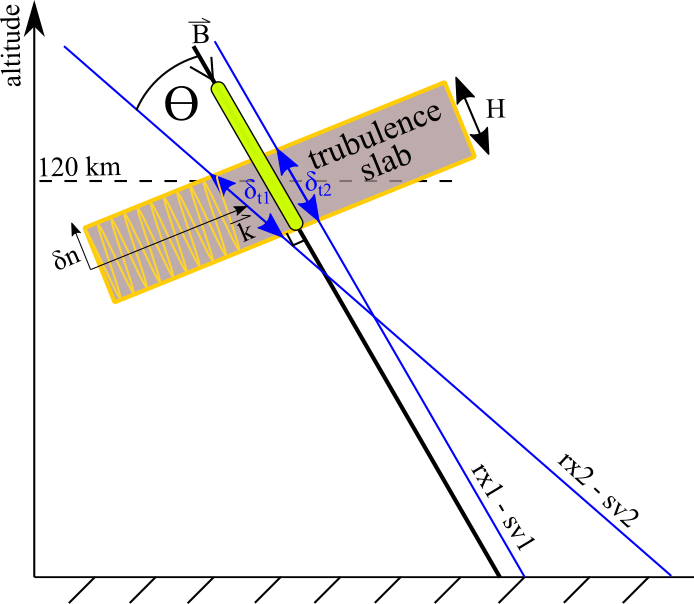
\includegraphics[width=.48\textwidth]{fig/turbulence}
\caption{Pictorial presentation of E-region turbulence probed by GNSS lines-of-sight, at an arbitrary angle.}
\label{fig:turbulence}
\end{wrapfigure}

Figure~\ref{fig:turbulence} illustrates geometry of multiple receivers, tracking different satellites in a presence of aurora. Green-shaded pill-like structure depicts auroral impact ionization and the corresponding optical emissions, elongated along the magnetic field lines. A region of plasma turbulence is depicted as a slab confined between 100 -- 130~km altitude~\citep{Dimant2011b}, with the irregularities' wave vector $\textbf{k}$ in $\textbf{k} \perp \textbf{B}$ direction.  

Two receiver's lines-of sight (blue lines) track two different satellites. While \textit{rx2 -- sv2} LOS is field aligned, \textit{rx1 -- sv1} probes the turbulence layer at a non-zero aspect angle $\Theta$. The aspect angle $\Theta$ denotes an angle between the geomagnetic inclination and the corresponding LOS direction. Assuming simple geometry of the turbulence slab with thickness $H$, and $\textbf{k} \perp \textbf{B}$~\citep{Chartier2016}, we assume the mapping function $F(\Theta)$ has a trigonometric nature with a correction coefficient $\alpha$: $F(\Theta)=\alpha \cdot \cos \Theta$. Therefore the probing length $\delta=\delta_0 / F(\Theta)$ is inversely proportional to the mapping function $F(\Theta)$, where $\delta_0$ is a turbulence thickness in field-aligned direction. Therefore, the observed scintillation depends on the aspect angle $\Theta$. We have a set of observations confirming the aspect angle dependence, however it is incomprehensive to estimate the relationship solely upon observations. Moreover, an elevation and azimuthal scan, done by a full 3D GNSS propagation model: Satellite-beacon Ionospheric-scintillation Global Model of the upper Atmosphere (SIGMA)~\citep{Key2014}, confirms the angular dependence. \textbf{A systematic approach, utilizing the 3D propagation model SIGMA~\citep{Key2014} is proposed to determine the mapping function. The modeling output will be then tested against the observations.}

\vspace{-0.5em}\subsection{Phase scintillation imaging and data fusion}

The final step is a 2D representation of individual phase scintillation observable on a geographical map. The procedure is similar to the global maps of TEC. We demonstrated a version of global maps produced by GNSS measurements for the 2017 total solar eclipse campaign\footnote{https://github.com/aldebaran1/pyTID}~\citep{Mrak2018eclipse, Mrak2018weather}. The imaging procedure, however, needs to be adjusted to different physical constraints, owing to observing different physical processes. In the case of the differential TEC imaging, the spatial scales are of an order of 100~km, while the auroral irregularities can be 2 orders of magnitude smaller. Therefore, we propose to engineer an optimal, physics constrained, 2D representation of plasma turbulence extracted by the GNSS phase scintillation observations.

Let alone, a line-of-sight phase scintillation measurement carries little contextual information. With a simultaneous 2D projection of many observations, one is able to add spatial dimensionality to the observing system. However, a physical interpretation ob the observations would rely of several physical assumptions. Fortunately, a peculiar nature of the high latitude MI-coupling enable utilization of optical aurora as a supporting, useful information-bearing signal, that can be used as a useful information to advance our knowledge of the phase scintillation. We propose and extend and exploit the GNSS-All sky imager (ASI) data fusion approach, developed for the Mahali campaign~\citep{Semeter2017,Mrak2018mahali}. We have utilized only the Poker Flat camera data to cover a small field-of-view. However, in order to extend the coverage we will utilize the Time History of Events and Mesoscale Interactions during Substorms (THEMIS) cameras\footnote{http://themis.ssl.berkeley.edu/instrument\_asi.shtml}. The GNSS-ASI data fusion will enable us to investigate, and relate the meso-scale MI coupling (optical aurora) with small-scale coupling (GNSS phase scintillation) in an unprecedented detail. 

% ----------------------------------------- Preliminary work ------------------------------------------------ %

\section{Phase scintillation localization and multi-sensor data fusion}

Preliminary work was based upon the "Mahali" project~\citep{Viktor2014}, a dedicated $\sim$15~km baseline GPS receiver array deployment, along roadways near the Poker Flat Research Range, central Alaska. We utilized the first ever GNSS receiver configuration of this kind in order to derive geophysical constraints in the measured phase scintillation. The main science objective concerns spatiotemporal localization geometry constraints in the phase scintillation. 

We utilized co-located optical and radar instrumentation in order to put the GNSS measurements into a proper context of a large-scale MI-coupled system. A data fusion approach, with a detailed sensor geometry and topology description was recently published~\citep{Mrak2018mahali,Semeter2017}. We have utilized a co-located Poker Flat All Sky Camera with a narrow band-pass filter centered at the $O(^1S)$ 557.7~nm emissions line, characteristic to the substorm particle precipitation with a dominating input energy range 1--10~keV~\citep{Banks1974}. In order to represent the different sensors on a common projection plane, we assumed the optical emission and the current closure resided in the ionospheric E- region at an altitude of 120~km.

\begin{wrapfigure}[23]{r}{0.5\textwidth}
\vspace{-1em}
\centering
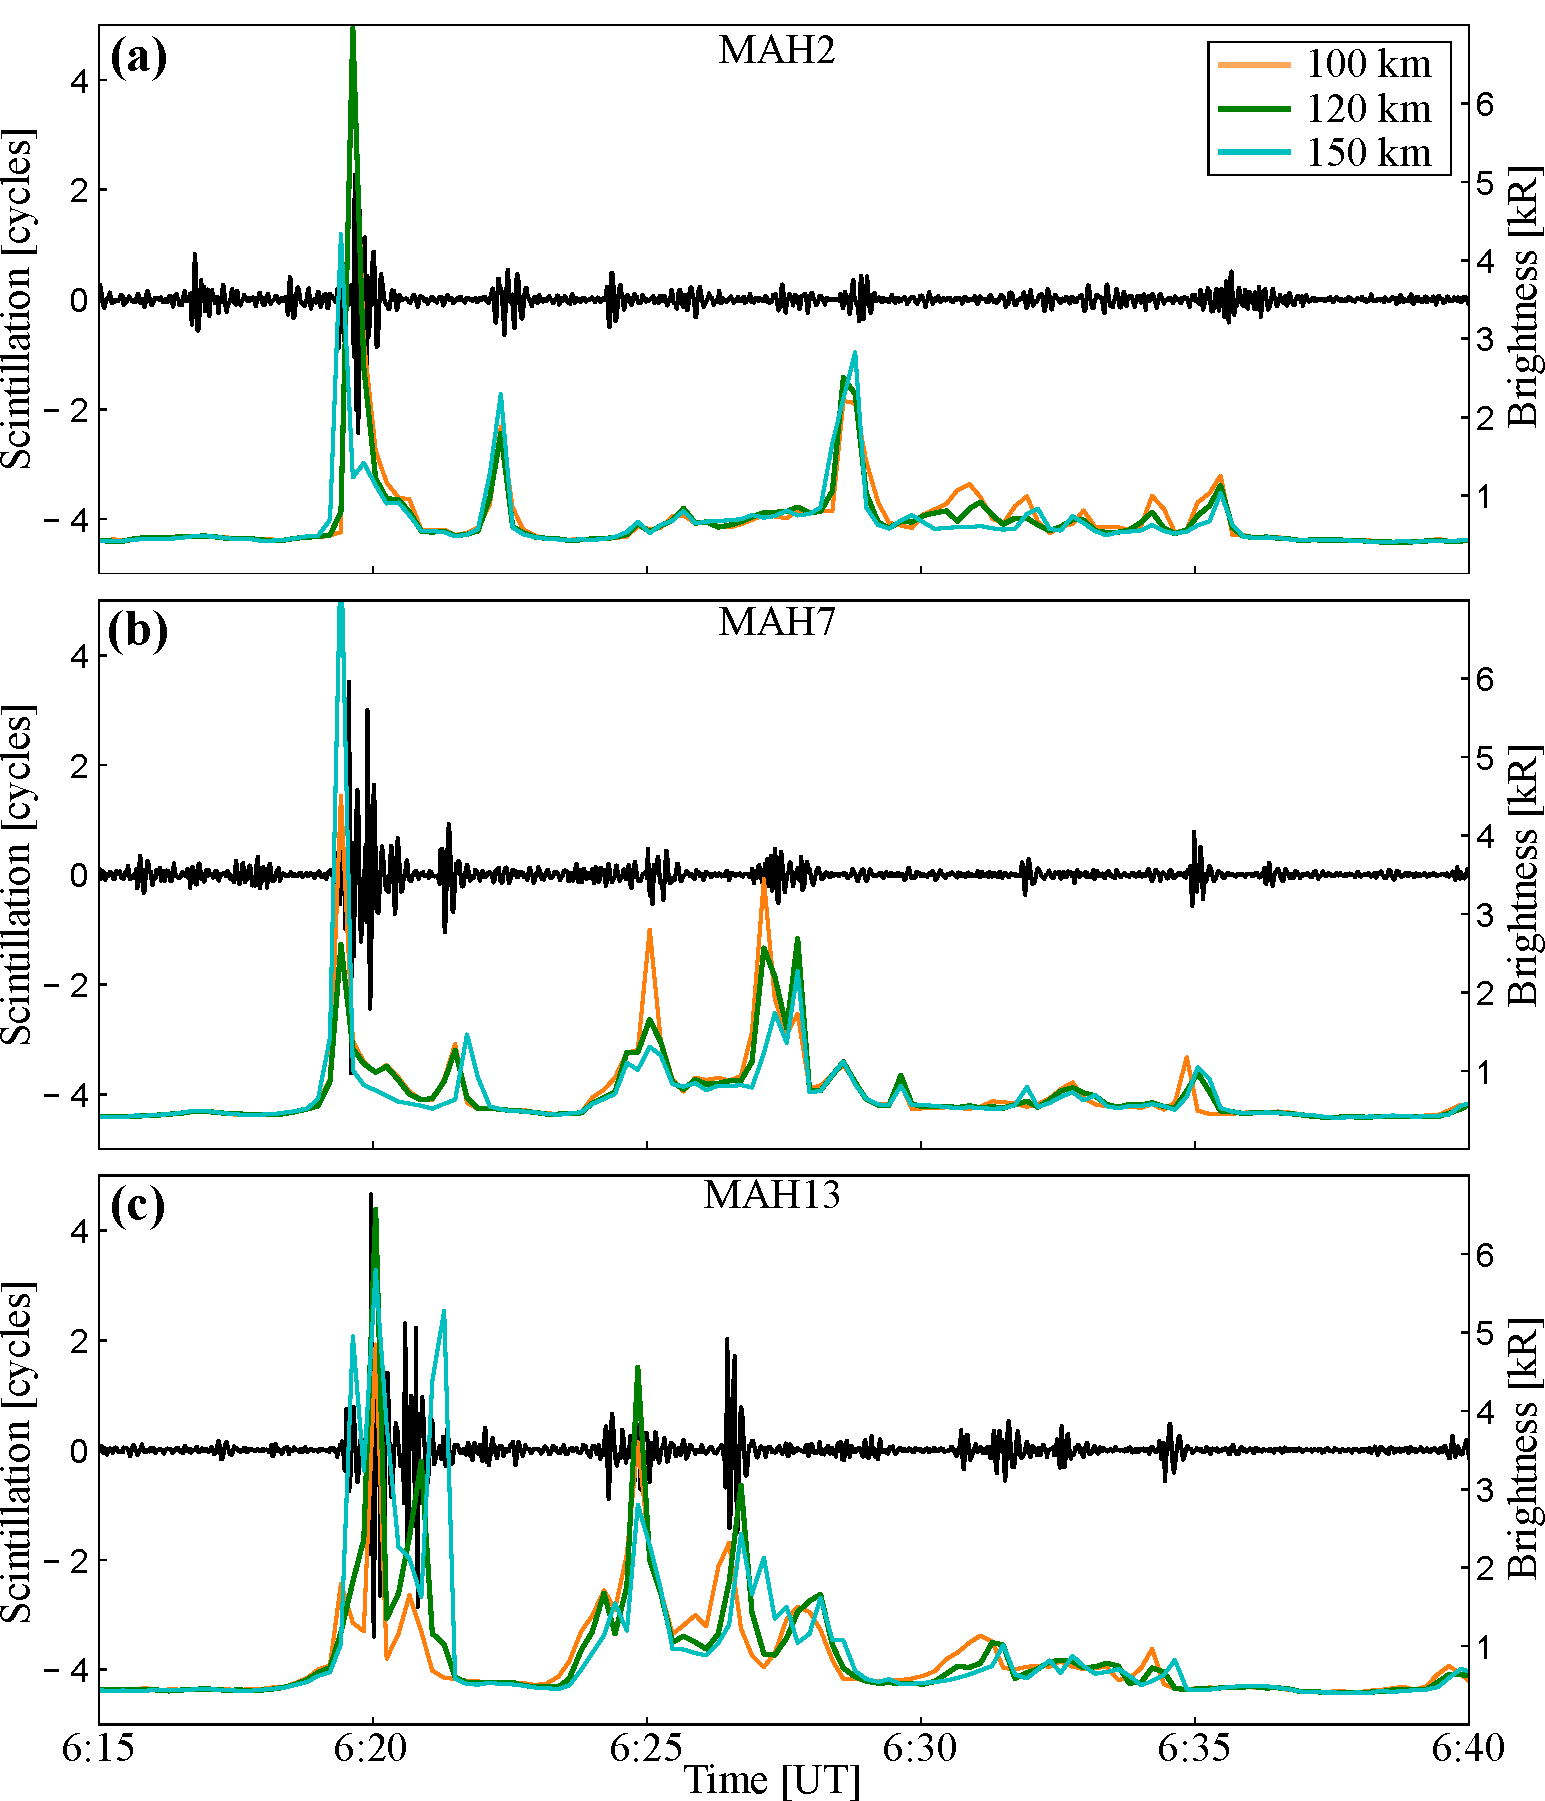
\includegraphics[width=0.45\textwidth]{fig/mapping}
\caption{Data fusion of GPS L1 scintillation (SV23) and the corresponding integrated green line brightness, using three different mapping assumptions: 100, 120 and 150~km altitude respectively. }
\label{fig:mapping}
\end{wrapfigure}

We test the spatial mapping ambiguity on three GPS receivers, employing the GPS-ASI data fusion at different mapping assumptions. We analyzed data from three GPS receivers and compared the extracted phase scintillation with the intercepted green line brightness for three different altitude assumptions: 100 km, 120 km, and 150 km. The results are shown in Figure~\ref{fig:mapping}. Receivers MAH2 and MAH13 were farthest away from the ASI, approximately 100~km away toward west and east, respectively. Receiver MAH7 was the closest but not co-located receiver to the ASI, approximately 15~km away (north-east). As shown in Figure~\ref{fig:mapping}, mapping uncertainties/deviations increase with baseline distance, showing almost no effect for the MAH7 receiver, and showing some notable differences at off-site receivers. However, the differences are relatively small, and have effectively no effect on the physical conclusions drawn from the observations. Therefore, considering the given sensor topology, observational geometry and mapping assumption analysis, we have used the 120~km mapping consistently throughout this work.

We analyze the data from the whole receiver array and find a persistent and persuasive pattern in the phase scintillation measurements, outlined in Figure~\ref{fig:mapping} for three receivers.
We find: 
\begin{itemize}[leftmargin=*]
\vspace{-0.5em}
\item GPS phase scintillation is correlated only with green line ($\lambda$557.7~nm) emission line, hence E-region structures/turbulence are the most likely source.
\vspace{-0.5em}
\item There is a notable correlation between amplitudes, however several outliers most likely indicate there is no direct correlation.
\vspace{-0.5em}
\item Duration of the phase scintillation and the arc brightness intensifications are not correlated.
\vspace{-0.5em}
\item Most intense scintillations are located on the edges of auroral brightness intensifications.
\vspace{-0.5em}
\item The phase scintillation does not depend on the total change in the TEC. The auroral precipitation events are not necessarily accompanied with phase scintillating structures. 
\vspace{-0.5em}
\item Observational geometry is an important factor, and it therefore constants the observations and the remote sensing field-of-view.
\end{itemize}

The new insights derived by means of concurrent observations and a careful data fusion approach suggest the source of the phase scintillation is a consequence of a highly complex and coupled electrodynamic system, controlled by the state of the MI-coupling. \textbf{The preliminary work directly addressed the science questions (a) and (b), and it laid down the fundamental physical constraints, enabled by the Mahali network and multi-sensor data fusion.} Similar conclusions were recently derived in terms of filed-aligned current system \citep{McGranaghan2017, Prikryl2016}. \textbf{Phase scintillation clustering on the edges of precipitation flux tubes can be linked to complex electrodynamics structures, however a complex geometry prevents a trivial 2D mapping of an arbitrary oriented GNSS observation. Therefore, in order to get a global view over small-scale plasma turbulence occurrence, we have to find an optimal way to utilize all available GNSS measurements.}

% ------------------------------------------------ Schedule ---------------------------------------------- %
\vspace{-0.5em}
\section{Schedule, milestones and anticipated contributions}

We endeavor to address the outstanding questions by virtue of leveraging the GNSS phase scintillation into a continental-scale plasma turbulence maps, and thus infer the state of the MI coupling in  unprecedented detail. The work flow is engineered in a way to fully encompass the observational geometry constraints, revealed by the preliminary work, and outlined by the outstanding question \textbf{(1)}. This tool will enable us to fully address the outstanding questions \textbf{(2)} and \textbf{(3)}. In a broader context, it will be a fundamental framework to build upon in order to exploit other outstanding question regarding the MI coupling. The outstanding questions \textbf{(2)} and \textbf{(3)} are a primary concern of the National Science Foundation Aeronomy - The Coupling, Energetics, and Dynamics of Atmospheric Regions (CEDAR) section.

\begin{figure}[h]
\centering
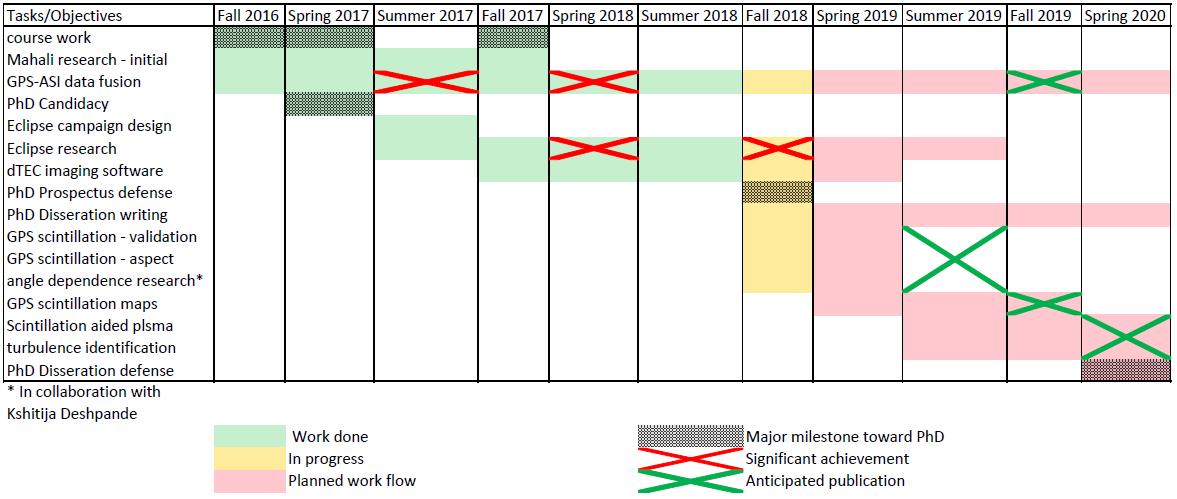
\includegraphics[width=\textwidth]{fig/progress.png}
\caption{PhD timeline with milestones and task and objectives. Green cells mark work that has been done, yellow cells are task that are underway, red cells are planned work. Overlays mark important milestones, including graduation milestones, publications, and anticipated contributions.}
\label{fig:progress}
\end{figure}
%
%The proposed schedule if depicted in Figure~\ref{fig:progress}. The milestones we aim to achieve are:\vspace{-0.5em}
%\begin{itemize}
%\item A thorough examination of small-scale to meso-scale interaction in the MI-coupling by virtue of concurrent phase scintillation and optical auroral observation.
%\vspace{-0.5em}
%\item An integration of available GNSS data into a phase scintillation imaging, including the full description of the newly derived mapping function.
%\vspace{-0.5em}
%\item Finally, we will utilize the GPS-ASI data fusion tool in order to derive an empirical climatology study of phase scintillation occurrence, and its connection to the geomagnetic drivers.
%\end{itemize}

\newpage
\bibliographystyle{plainnat}
\begin{thebibliography}{99}
\small
\bibitem[{\textit{Appleton and Chapman}}(1932)]{Appleton1932}
Appleton, E. V., and F. W. Chapman (1932), The collisional friction experienced by vibrating electrons in ionized air (1931), \emph{Proceedings of the Physical Society}, 44-3.
\vspace{-1em}
\bibitem[{\textit{Banks et~al.}}(1974)]{Banks1974}
Banks, P. M., C. R. Chappell, and A. F. Nagy (1974), A new model for the interaction of auroral electrons with the atmosphere: Spectral degradation, backscatter, optical emission, and ionization, \emph{J. Geophys. Res.}, 79(10), 1459–1470, doi: 10.1029/JA079i010p01459. 
\vspace{-1em}
\bibitem[{\textit{Chartier et~al}}(2016)]{Chartier2016}
Chartier, A., B. Forte, K. Deshpande, G. Bust, and C. Mitchell (2016), Three-dimensional modeling of high-latitude scintillation observations, \textit{Radio Sci.}, 51, 1022-1029, doi:10.1002/2015RS005889.
\vspace{-1em}
\bibitem[{\textit{Coster et~al.}}(1992)]{Coster1992}
Coster, A., J., Gaposchkin, E., M., and Thornton, L., E., (1992), Real-Time Ionospheric Monitoring System Using GPS, \textit{Journal of The Institute of Navigation}, 38, 2, doi:10.1002/j.2161-4296.1992.tb01874.x.
\vspace{-1em}
\bibitem[{\textit{Coster et~al.}}(2012)]{Coster2012}
Coster, A., D. Herne, P. Erickson, and D. Oberoi (2012), Using the Murchison Widefield Array to observe midlatitude space weather, \emph{Radio Sci.}, 47, RS0K07, doi:10.1029/2012RS004993.
\vspace{-1em}
\bibitem[{\textit{Deshpande et~al.}}(2014)]{Key2014}
Deshpande, K. B., G. S. Bust, C. R. Clauer, C. L. Rino, and C. S. Carrano (2014), Satellite-beacon Ionospheric-scintillation Global Model of the upper Atmosphere (SIGMA) I: High-latitude sensitivity study of the model parameters, \emph{J. Geophys. Res. Space Physics}, 119, 4026-4043, doi:10.1002/2013JA019699.
\vspace{-1em}
\bibitem[{\textit{Dimant and Milikh}}(2003)]{Dimant2003}
Dimant, Y. S., and G. M. Milikh, Model of anomalous electron heating in the E region: 1. Basic theory, \emph{J. Geophys. Res.}, 108(A9), 1350, doi:10.1029/2002JA009524, 2003.
\vspace{-1em}
\bibitem[{\textit{Dimant and Oppenheim}}(2011a)]{Dimant2011a}
Dimant, Y. S., and M. M. Oppenheim (2011), Magnetosphere‐ionosphere coupling through E region turbulence:
1. Energy budget, J. Geophys. Res., 116, A09303, doi:10.1029/2011JA016648.
\vspace{-1em}
\bibitem[{\textit{Dimant and Oppenheim}}(2011b)]{Dimant2011b}
Dimant, Y. S., and M. M. Oppenheim (2011), Magnetosphere‐ionosphere coupling through E region turbulence:
2. Anomalous conductivities and frictional heating, \emph{J. Geophys. Res.}, 116, A09304, doi:10.1029/2011JA016649.
\vspace{-1em}
\bibitem[{\textit{Foster et~al.}}(2002)]{Foster2002}
Foster, J. C., P. J. Erickson, A. J. Coster, J. Goldstein, and F. J. Rich (2002), Ionospheric signatures of plasmaspheric tails, \emph{Geophys. Res. Lett.}, 29(13), doi:10.1029/2002GL015067.
\vspace{-1em}
\bibitem[{\textit{Foster et~al.}}(2005)]{Foster2005}
Foster, J. C., et al. (2005), Multiradar observations of the polar tongue of ionization, \emph{J. Geophys. Res.}, 110, A09S31, doi:10.1029/2004JA010928.
\vspace{-1em}
\bibitem[{\textit{Fremouw et~al.}}(1978)]{Fremouw1978}
Fremouw, E. J., R. L. Leadabrand, R. C. Livingston, M. D. Cousins, C. L. Rino, B. C. Fair, and R. A. Long (1978), Early results from the DNA wideband satellite experiment-Complex-signal scintillation, \emph{Radio Sci.}, 13(1), 167-187, doi:10.1029/RS013i001p00167.
\vspace{-1em}
\bibitem[{\textit{Jacobsen and Andalsvik}}(2016)]{Jacobsen2016}
Jacobsen, K. S., and Y. L. Andalsvik (2016). Overview of the 2015 St. Patrick’s day storm and its consequences for RTK and PPP positioning in Norway \emph{J. Space Weather Space Clim.}, 6 - A9 DOI: 10.1051/swsc/2016004.
\vspace{-1em}
\bibitem[{\textit{Jiao et~al}}(2013)]{Jiao2013}
Jiao, Y., Y. T. Morton, S. Taylor, and W. Pelgrum (2013), Characterization of high-latitude ionospheric scintillation of GPS signals, \textit{Radio Sci.}, 48, 698-708, doi:10.1002/2013RS005259.
\vspace{-1em}
\bibitem[{\textit{Kashcheyev et~al.}}(2012)]{Kashcheyev2012}
Kashcheyev, A., B. Nava, and S. M. Radicella (2012), Estimation of higher-order ionospheric errors in GNSS
positioning using a realistic 3-D electron density model, Radio Sci., 47, RS4008, doi:10.1029/2011RS004976.
\vspace{-1em}
\bibitem[{\textit{McGranaghan et~al.}}(2017)]{McGranaghan2017}
McGranaghan, R. M., Mannucci, A. J., \& Forsyth, C. (2017). A comprehensive analysis of multiscale field‐aligned currents: Characteristics, controlling parameters, and relationships. \emph{J. Geophys. Res. Space Physics}, 122, 11,931–11,960. https://doi.org/10.1002/2017JA024742.
\vspace{-1em}
\bibitem[{\textit{Mitchell et~al.}}(2005)]{Mitchell2005}
Mitchell, C. N., L. Alfonsi, G. De Franceschi, M. Lester, V. Romano, and A. W. Wernik (2005), GPS TEC and scintillation measurements from the polar ionosphere during the October 2003 storm, \emph{Geophys. Res.
Lett.}, 32, L12S03, doi:10.1029/2004GL021644.
\vspace{-1em}
\bibitem[\textit{Mrak et~al.}(2018a)]{Mrak2018mahali} 
Mrak, S., et al., (2018), Field-aligned GPS Scintillation: Multi-Sensor Data Fusion, \emph{J. Geophys. Res. Space Physics}, 123, doi:10.1002/2017JA024557.
\vspace{-1em}
\bibitem[\textit{Mrak et~al.}(2018b)]{Mrak2018eclipse}
Mrak, S., Semeter, J. L., Drob, D., \& Huba, J. D. (2018). Direct EUV/X-ray modulation of the ionosphere during the August 2017 total solar eclipse. \emph{Geophysical Research Letters}, 45. https://doi.org/10.1029/2017GL076771.
\vspace{-1em}
\bibitem[\textit{Mrak et~al.}(2018c)]{Mrak2018weather}
Mrak, S., Semeter, J. L., Nishimura, Y., Hirsch, \& M., Sivadas, N. (2018). Coincidental TID Production by Tropospheric Weather during the August 2017 Total Solar Eclipse. \emph{Geophysical Research Letters}, doi:10.1029/2018GL080239.
\vspace{-1em}
\bibitem[{\textit{Pankratius et~al.}}(2014)]{Viktor2014}
Pankratius, V., F. Lind, A. Coster, P. Erickson and J. Semeter (2014), Mobile crowd sensing in space weather monitoring: the mahali project, \textit{IEEE Communications Mag.}, 	Vol: 52, Issue: 8, doi:10.1109/MCOM.2014.6871665.
\vspace{-1em}
\bibitem[{\textit{Prikryl et~al}}(2011)]{Prikryl2011}
Prikryl, P., Jayachandran, P. T., Mushini, S. C., and Chadwick, R.: Climatology of GPS phase scintillation and HF radar backscatter for the high-latitude ionosphere under solar minimum conditions, Ann. Geophys., 29, 377-392, https://doi.org/10.5194/angeo-29-377-2011, 2011. 
\vspace{-1em}
\bibitem[{\textit{Prikryl et~al.}}(2016)]{Prikryl2016}
Prikryl, P., et al. (2016), GPS phase scintillation at high latitudes during the geomagnetic storm of 17–18 March 2015, \emph{J. Geophys. Res. Space Physics}, 121, 10,448–10,465, doi: 10.1002/2016JA023171. 
\vspace{-1em}
\bibitem[{\textit{Rideout and Coster}}(2006)]{Rideout2006}
Rideout, W., and Coster, A., (2006), Automated GPS processing for global total electron content data, \textit{GPS Solutions}, 10:219. doi:10.1007/s10291-006-0029-5.
\vspace{-1em}
\bibitem[{\textit{Semeter et~al}}(2017)]{Semeter2017}
Semeter, J., S. Mrak, et.al. (2017), GPS signal corruption by the discrete Aurora: Precise measurements from the Mahali experiment, \textit{Geophys. Res. Lett.}, 44, 9539-9546, doi:10.1002/2017GL073570.
\vspace{-1em}
\bibitem[{\textit{Spogli et~al.}}(2009)]{Spogli2009}
Spogli, L., Alfonsi, L., De Franceschi, G., Romano, V., Aquino, M. H. O., and Dodson, A. (2009), Climatology of GPS ionospheric scintillations over high and mid-latitude European regions, \textit{Ann. Geophys.}, 27, 3429-3437, doi:10.5194/angeo-27-3429-2009.
\vspace{-1em}
\bibitem[{\textit{van der Meeren et~al.}}(2015)]{vanderMeeren2015}
van der Meeren, C., K. Oksavik, D. A. Lorentzen, M. T. Rietveld, and L. B. N.Clausen (2015), Severe and localized GNSS scintillation at the poleward edge of the nightside auroral oval during intense sub-storm aurora, \textit{J.Geophys. Res. Space Physics}, 120, 10, 607-10, 621, doi:10.1002/2015JA021819.
\vspace{-1em}
\bibitem[{\textit{Wiltberger et~al.}}(2017)]{Wiltberger2017}
Wiltberger, M., et al. (2017), Effects of electrojet turbulence on a magnetosphere-ionosphere simulation of a geomagnetic storm, \emph{J. Geophys. Res. Space Physics}, 122, 5008-5027, doi:10.1002/2016JA023700.
\vspace{-1em}

\end{thebibliography}

\end{document}
